%%------------------------------------
%% This is for the workbook 
%% tar -cvf work.tar *.tex ./Fig*/*.fig
%%
%% To make the book
%% unix% latex work.tex
%% unix% makeindex work
%% unix% latex work.tex
%% unix% dvips work.dvi -o work.ps
%% unix% ghostview work.ps &
%%
%%------------------------------------

%% Author:      Chris Coulston
%% Purp:        Here are the homework problems and their solutions.

%%\documentclass[11pt,psfig]{book}
\documentclass[letterpaper, 10pt]{memoir}
\chapterstyle{ger}
\settrims{0pt}{0pt}
\semiisopage[9]		% [N] is spine margin is 1/Nth pf page 


% To keep the book.tex file clean, I pulled all the formating and package 
% includes into the preamble.tex file
%%------------------------------------------------------
%%------------------------------------------------------

\usepackage{amsmath,amssymb}
\usepackage{lmodern}
\usepackage{iftex}

\usepackage{xcolor}
\usepackage{graphicx}

\usepackage{dirtree}		% For the body of knowledge


\usepackage{listings}

\makeatletter
\def\maxwidth{\ifdim\Gin@nat@width>\linewidth\linewidth\else\Gin@nat@width\fi}
\def\maxheight{\ifdim\Gin@nat@height>\textheight\textheight\else\Gin@nat@height\fi}
\makeatother
% Scale images if necessary, so that they will not overflow the page
% margins by default, and it is still possible to overwrite the defaults
% using explicit options in \includegraphics[width, height, ...]{}
\setkeys{Gin}{width=\maxwidth,height=\maxheight,keepaspectratio}
% Set default figure placement to htbp
\makeatletter
\def\fps@figure{htbp}
\makeatother

\usepackage{longtable,booktabs,array}
\usepackage{multirow}
\usepackage{calc}
\usepackage[normalem]{ulem}

\usepackage{pdflscape}

\usepackage{bookmark}

\usepackage{xurl}

\usepackage{hyperref}

%\let\oldhypertarget\hypertarget
%\renewcommand*{\hypertarget}{\oldhypertarget\space}



\hypersetup{
   colorlinks=true,
   linkcolor=red}

\makeindex

\begin{document}


\frontmatter
 \title{Digital Design, A Datapath and Control Approach - The Workbook}
 \author{Chris Coulston}
 \date{}
 \maketitle

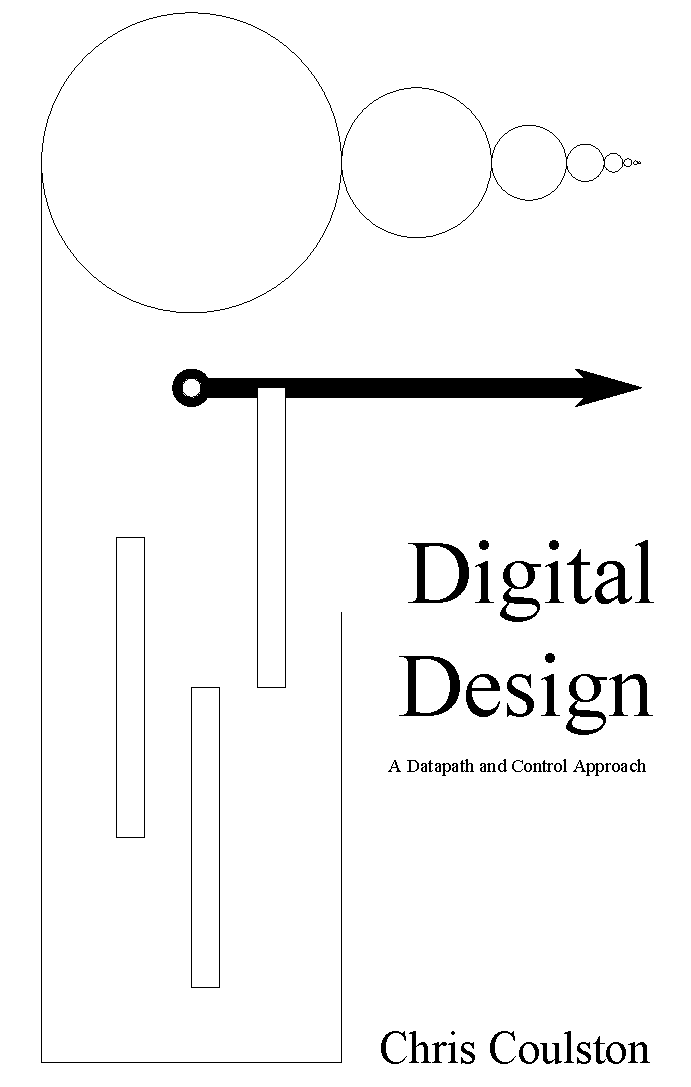
\includegraphics{./Fig/cover}
\showanswers
%%\hideanswers 

\tableofcontents
\mainmatter

\chapter{Numbering Systems}
\label{chapter:NumberingSystems}
\graphicspath{ {./chapter01/Fig} }

\subsection{Helpfull Stuff}

\begin{tabular}{|c|c|c|c|}\hline
Decimal & Binary & Hexadecimal \\ \hline
0	& 0000	& 0	 \\ \hline
1	& 0001	& 1	 \\ \hline
2	& 0010	& 2	 \\ \hline
3	& 0011	& 3	 \\ \hline
4	& 		& 4	 \\ \hline
5	& 0101	& 5	 \\ \hline
6	& 		& 6	 \\ \hline
7	& 		& 7	 \\ \hline
8	& 1000	& 8	 \\ \hline
9	& 		& 9	 \\ \hline
10	& 1010	& A	 \\ \hline
11	& 		& B	 \\ \hline
12	& 1100	& C	 \\ \hline
13	& 1101	& D	 \\ \hline
14	& 		& E	 \\ \hline
15	& 1111	& F	 \\ \hline
\end{tabular}
\vspace{0.5in}

\begin{tabular}{|c|c|c|c|c|c|c|c|c|c|c|}\hline
i    & 0 & 1 &  2 &  3 &  4 &  5 &  6 &  7  &  8  &  9  \\ \hline
$2^i$ & 1 & 2 &  4 &  8 & 16 & 32 & 64 & 128 & 256 &  512\\ \hline
\end{tabular}
\vspace{0.5in}

{\tiny
$\begin{array}{l}
1110101011_2= \\
1*2^9+1*2^8+1*2^7+0*2^6+1*2^5+0*2^4+1*2^3+0*2^2+1*2^1+1*2^0 = \\
2^8(0*2^3+0*2^2+1*2^1+1*2^0) + 2^4(1*2^3+0*2^2+1*2^1+0*2^0) + 2^0*(1*2^3+0*2^2+1*2^1+1*2^0) =\\
2^8(0011_2) + 2^4(1010_2) +  2^0(1011_2) =\\
2^{4*2}(0011_2) + 2^{4*1}(1010_2) +  2^{4*0}(1011_2) =\\
16^2(0011_2) + 16^1(1010_2) + 16^0*(1011_2) =\\
16^2(3) + 16^1(A) + 16^0*(B) =\\
3AB_{16}
\end{array}$
}


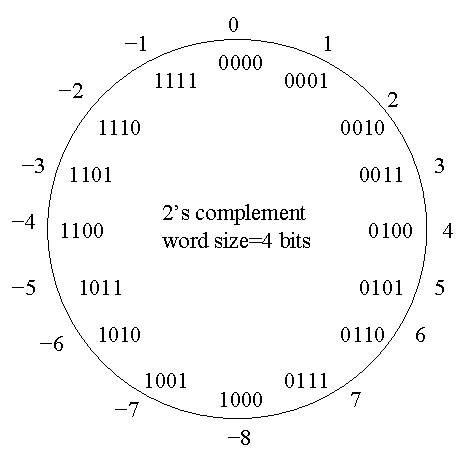
\includegraphics{2wheel}




\end{document} 
